\chapter{Controller Design}\label{chap:Control}
The system of the quadcopter has been described by a mathematical model, that is to be used in the design of a control system. The control system must stabilize the naturally unstable system of the quadcopter. It should also meet the functional requirements stated in \autoref{ch:functionalRequirements}.

The model can be divided into two submodels, an attitude model and a translational model. It is therefore desirable to design two control systems, one for each model. The attitude controller forms an inner loop surrounded by the translational x and y controllers and the z controller handles the amount of thrust applied by the motors by changing the retired sum of their rotational speeds. \autoref{fig:ControlHeadDiagram} shows the relation between the different controllers in the system.
\begin{figure}[H]
	\centering
	\includegraphics[width=1 \textwidth]{figures/generalcontroldiagram}
	\caption{Block diagram of overall control system.}
	\label{fig:ControlHeadDiagram}
\end{figure}
\fxnote{Explain what is the rotational speed calculation}

\autoref{fig:ControlHeadDiagram} is a block diagram of the overall control system.
The attitude controller is an inner controller and is designed as state space, as this allows multiple inputs. The three angles roll, pitch and yaw are coupled and therefore complex to control individually, as the single controllers will disturb each other resulting in a less effective control system. The translational control system is going to be designed with classical control principles, where bode plots and root locus are the design method to obtain proportional controllers. 

First the design of the attitude controller is done followed by the design of the translational controller. 
When the controllers are designed, they are simulated with the linear models to ensure, that the controllers yield the desired behavior. Afterwards the controllers are simulated with the models, that are not linearized, as these represent the true behavior of the plant. If the controllers yield an acceptable outcome, they are to be implemented in the system. To do so, they are first discretized. It is necessary to simulate the discrete controllers and compare the results with the continuous controllers, as some design considerations may be lost in the discretization. Lastly the controllers are implemented on the micro controller and the system is to be tested in the Vicon room. 